\section{问题一：数据质量评价、冲突消解与领域配比建模}

\subsection{质量指标的预处理与标量化}

附件 A 的 22 个指标中，14 个是标量、8 个是列表型。列表型必须先压缩为标量。按各指标的原始语义分别处理：

\begin{itemize}[leftmargin=2em,itemsep=2pt]
\item \texttt{fineweb\_edu} 为单元素列表，直接取该元素。
\item \texttt{modernbert\_cleanliness/readability/reasoning/professionalism} 为六分类 logits，本文取 $\arg\max/5$ 作为等级得分，使取值落入 $[0,1]$；作为敏感性对照另做了 softmax 期望 $\mathbb{E}[c]=\sum_c p_c\,c/5$。
\item \texttt{fluency\_en} 为二分类 logits，取 softmax 后流畅类的概率。
\item \texttt{ad\_en} 的官方类别顺序为 $[\text{has\_ad},\text{no\_ad}]$，取第二类（无广告）的 softmax 概率，该值本身已是正向。
\item \texttt{qurater} 是四个语义子维度的评分而非分类 logits，不能做 softmax。本文对四个维度各自做标准化后取平均，避免量纲差异主导。
\item 8 个 \texttt{rps\_*} 指标为标量，按各自语义处理。
\end{itemize}

\subsection{方向统一与稳健归一化}

题面要求把所有指标统一为``越高越好''。本文的处理分两步，顺序不能颠倒：

先在\textbf{冻结的参考集}（A1 抽样集）上估计归一化参数：对每个指标取 1\% 与 99\% 分位作为截尾边界，再线性映射到 $[0,1]$，即

\begin{equation}
U_{im}=\mathrm{clip}\!\left(\frac{x_{im}-\ell_m}{h_m-\ell_m},\,0,\,1\right),
\end{equation}

其中 $\ell_m,h_m$ 为指标 $m$ 的 1\%/99\% 分位。截尾是为了避免个别极端值把整个尺度压缩。该参数一经确定即应用于 A2/A3，\textbf{不对每个域分别做分位数变换}——否则域间的高低比较将失去意义。

再对\textbf{明确负向}的指标做补转换 $U\leftarrow1-U$。本文识别出 6 个负向指标：\texttt{ad\_en}（广告）、\texttt{rps\_doc\_frac\_chars\_top\_2gram} 与 \texttt{\_top\_3gram}（n-gram 重复率）、\texttt{rps\_lines\_uppercase\_letter\_fraction}（大写行占比）、\texttt{rps\_doc\_frac\_no\_alph\_words}（非字母词占比）、\texttt{rps\_lines\_numerical\_chars\_fraction}（数字字符占比）。

有一类指标需要特别处理：\texttt{rps\_doc\_word\_count}（词数）与 \texttt{rps\_doc\_num\_sentences}（句数）并非单调越好——过短说明信息量不足，过长往往是未清洗的拼接文本。本文对这两个指标采用倒 U 型效用，峰位设在归一化后的 0.35 处：

\begin{equation}
U \leftarrow 1-\frac{|U-0.35|}{\max(0.35,\,0.65)} .
\end{equation}

\subsection{分层综合质量评分模型}

\subsubsection{语义分组}

按 SlimPajama-Meta-rater 数据卡的指标语义，将 22 个指标分为 4 组：

\begin{table}[htbp]
\centering
\caption{质量语义分组}
\label{tab:qgroups}
\small
\begin{tabular}{c|l|l}
\toprule
\textbf{组别} & \textbf{含义} & \textbf{包含指标} \\
\midrule
教育价值 & 文本的知识密度与学习价值 & 教育价值、DSIR 书籍/百科/数学、质量评分、推理性 \\
可读性 & 语言流畅与结构清晰 & 可读性、洁净度、流畅度、一元熵 \\
专业性 & 术语规范与表达严谨 & 专业性、平均词长、唯一词比 \\
低噪声 & 广告、重复与格式噪声 & 无广告、非字母词比、2/3-gram 重复、大写行比、终止标点比、数字字符比、词数、句数 \\
\bottomrule
\end{tabular}
\end{table}

\subsubsection{组内平均与组间几何平均}

对样本 $i$，先取组内算术平均得 $z_{ig}$，再取组间几何平均得基础质量分：

\begin{equation}
Q_i^{\mathrm{base}}=\left(\prod_{g=1}^{4}\left(z_{ig}+\varepsilon\right)\right)^{1/4}-\varepsilon,
\qquad \varepsilon=10^{-3}.
\end{equation}

选几何平均而非算术平均，是因为几何平均对短板敏感：只要有一个组得分很低，整体得分就会被显著拉低，这与``教材存在明显缺陷时整体质量不高''的判断一致。$\varepsilon$ 用于避免零值导致对数发散，其取值在 $10^{-4}\sim10^{-2}$ 范围内对结果排序几乎无影响（敏感性见\ref{sec:q1_sens}节）。

图~\ref{fig:q1_corr} 给出 22 个指标的相关结构与语义分组。可以看出同组指标普遍正相关，但组间相关性较弱甚至为负——尤其``教育价值''与``低噪声''两组几乎不相关，这正是冲突产生的结构性原因。

\begin{figure}[htbp]
\centering
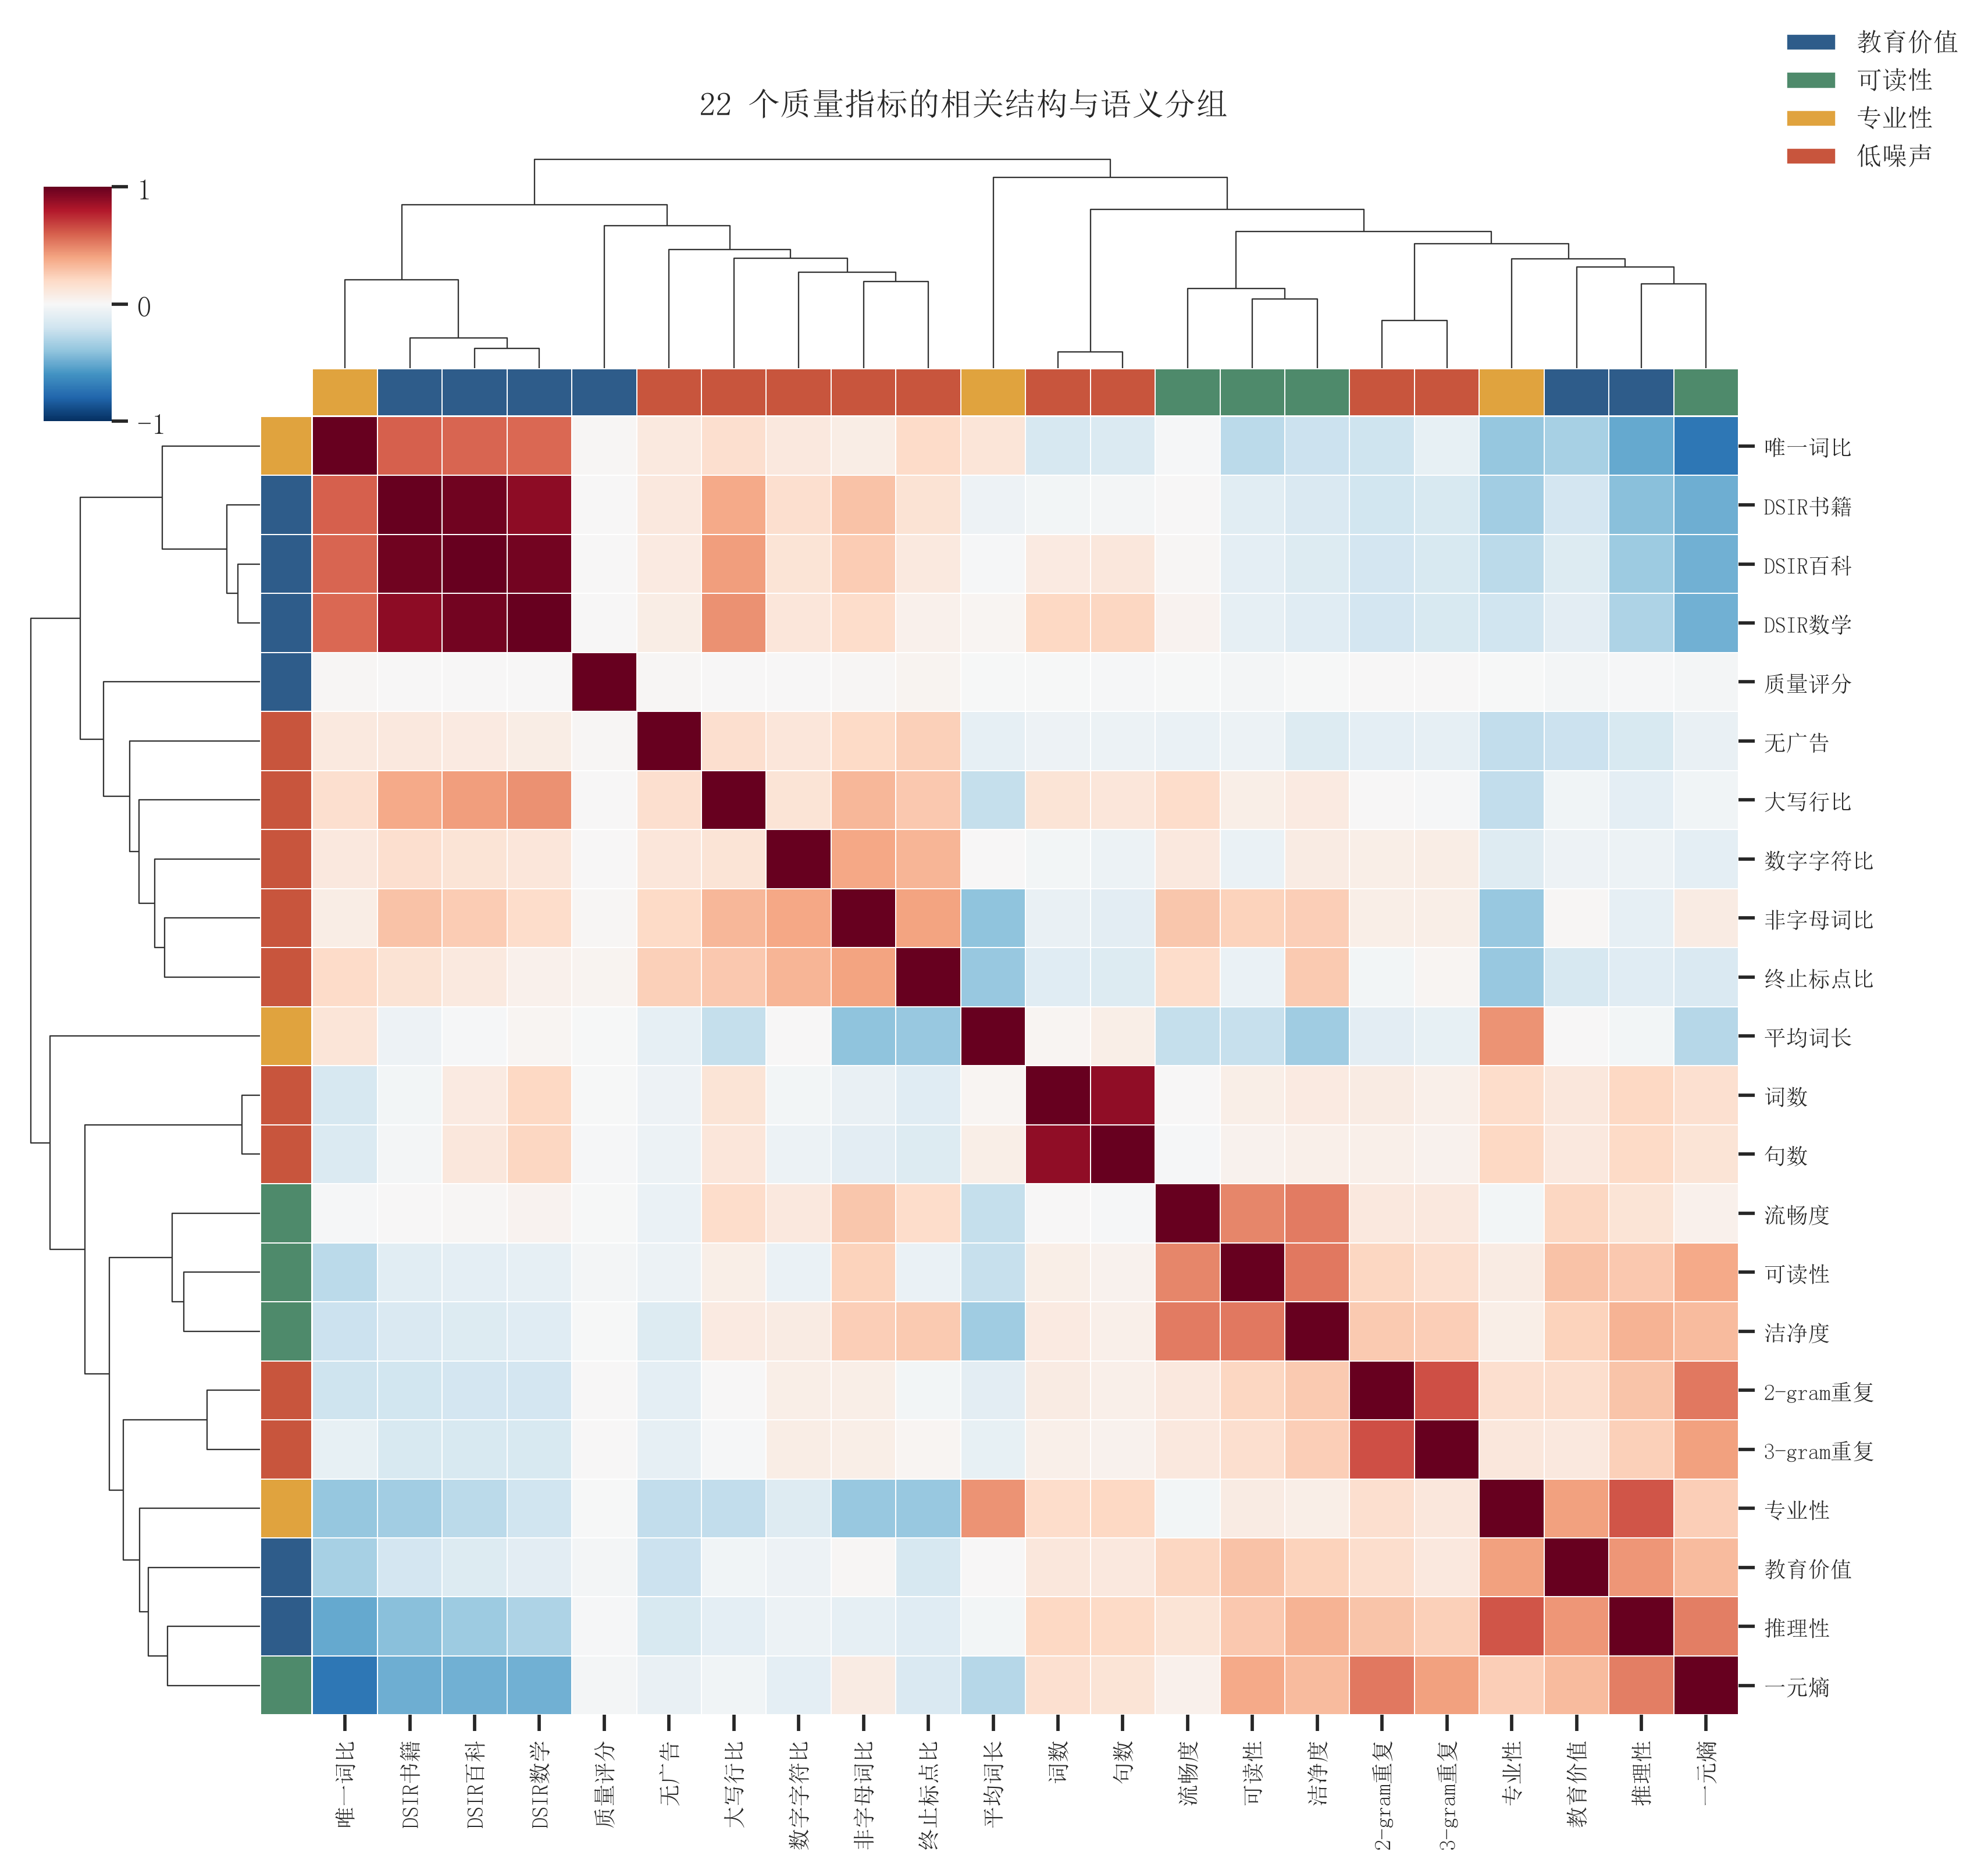
\includegraphics[width=0.78\textwidth]{figures/fig_q1_metric_corr.png}
\caption{质量指标相关结构与分组}
\label{fig:q1_corr}
\end{figure}

\subsection{质量冲突的定义、成因与消解}

\subsubsection{冲突的数学定义}

设 $z_{ig}$ 为样本 $i$ 在第 $g$ 组的得分。本文把冲突强度定义为组间极差：

\begin{equation}
c_i=\max_{g}z_{ig}-\min_{g}z_{ig}.
\label{eq:conflict}
\end{equation}

选极差而非方差，是因为极差直接对应``最好的维度与最差的维度相差多少''，量纲与 $Q$ 一致、易于解释，且不受组数影响。阈值 $\tau$ 由开发参考集上 $c$ 的 75\% 分位确定，得 $\tau=0.577$；$c_i>\tau$ 标记为冲突样本。本文另做了多个阈值的敏感性分析。

需要强调的是：\textbf{范围差只能发现不一致，不能证明某一指标错误}。文本确实可能同时``信息密度高''与``格式噪声大''（论坛长帖、代码注释），这属于真实特征而非测量错误。

\subsubsection{冲突的成因剖析}

图~\ref{fig:q1_conflict} 展示了冲突的结构。左图是教育价值与低噪声两组的联合分布，散点沿对角线两侧明显铺开，说明两者相关性很弱。中图给出各域冲突率：StackExchange 仅 0.24\%，而 book 域高达 83.3\%。右图把冲突归纳为五类典型模式。

\begin{figure}[htbp]
\centering
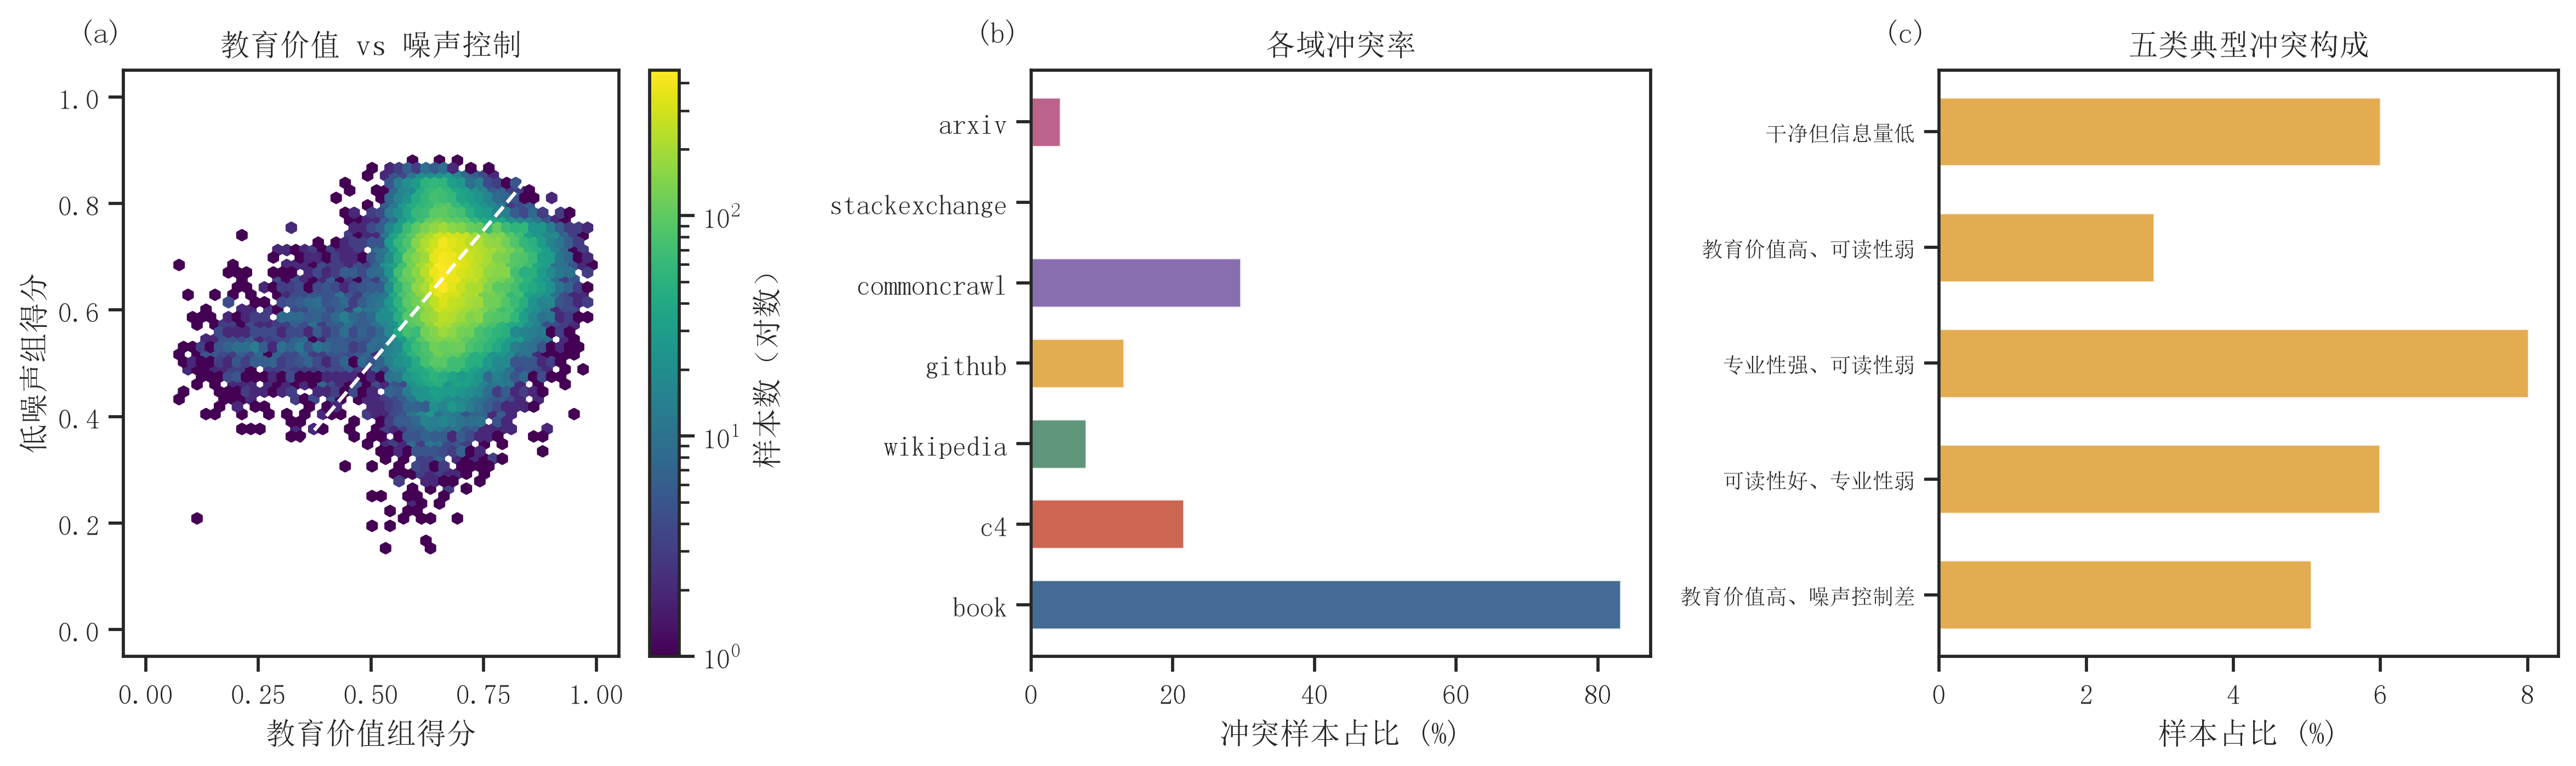
\includegraphics[width=0.95\textwidth]{figures/fig_q1_conflict.png}
\caption{质量冲突的结构与典型模式}
\label{fig:q1_conflict}
\end{figure}

冲突率在域间的巨大差异说明\textbf{冲突主要是体裁特征而非测量故障}。book 域多为扫描或早期数字化的长文本，教育价值评分高但格式规范性差、非字母字符比例高，因而``教育价值高、噪声控制差''这一类冲突占比最高。这一解释与图~\ref{fig:q1_conflict}(c) 中该类型占比最大相互印证。

\subsubsection{消解规则}

本文采用基础分与最弱组的凸组合：

\begin{equation}
Q_i^{(\lambda)}=(1-\lambda)\,Q_i^{\mathrm{base}}+\lambda\min_g z_{ig},
\qquad 0\le\lambda\le1 .
\label{eq:resolve}
\end{equation}

$\lambda=0$ 即不处理冲突（消融对照），$\lambda$ 越大越强调短板约束。$\lambda$ 由小规模预设网格 $\{0,0.1,\dots,0.5\}$ 确定，本文取 $\lambda=0.3$。图~\ref{fig:q1_inter}(b) 给出 $\lambda$ 的影响：随 $\lambda$ 增大，质量分均值由 0.557 单调降至 0.433，但与 $\lambda=0$ 结果的 Spearman 秩相关仍高达 0.966，说明消解规则改变了分数的绝对水平却基本保持了排序，是一个``温和''的修正。

该规则满足一个必要的一致性要求：若单独改善某一指标，$Q$ 不会下降。

\subsection{质量评分结果}

\subsubsection{域级质量}

表~\ref{tab:q1_dom} 与图~\ref{fig:q1_dist}、图~\ref{fig:q1_dom} 给出域级结果。

\begin{table}[htbp]
\centering
\caption{七个质量域的域级质量与冲突率}
\label{tab:q1_dom}
\small
\begin{tabular}{l|r|r|r|r|r}
\toprule
\textbf{域} & \textbf{样本数} & \textbf{平均 $Q$} & \textbf{2.5\%分位} & \textbf{97.5\%分位} & \textbf{冲突率} \\
\midrule
arxiv         & 2\,360  & \textbf{0.589} & 0.482 & 0.651 & 4.2\% \\
stackexchange & 1\,690  & 0.552 & 0.421 & 0.644 & 0.2\% \\
commoncrawl   & 26\,700 & 0.482 & 0.337 & 0.633 & 29.6\% \\
github        & 2\,660  & 0.479 & 0.254 & 0.626 & 13.2\% \\
wikipedia     & 1\,940  & 0.475 & 0.331 & 0.621 & 7.8\% \\
c4            & 13\,700 & 0.474 & 0.299 & 0.633 & 21.6\% \\
book          & 1\,362  & \textbf{0.312} & 0.100 & 0.535 & \textbf{83.3\%} \\
\bottomrule
\end{tabular}
\end{table}

\begin{figure}[htbp]
\centering
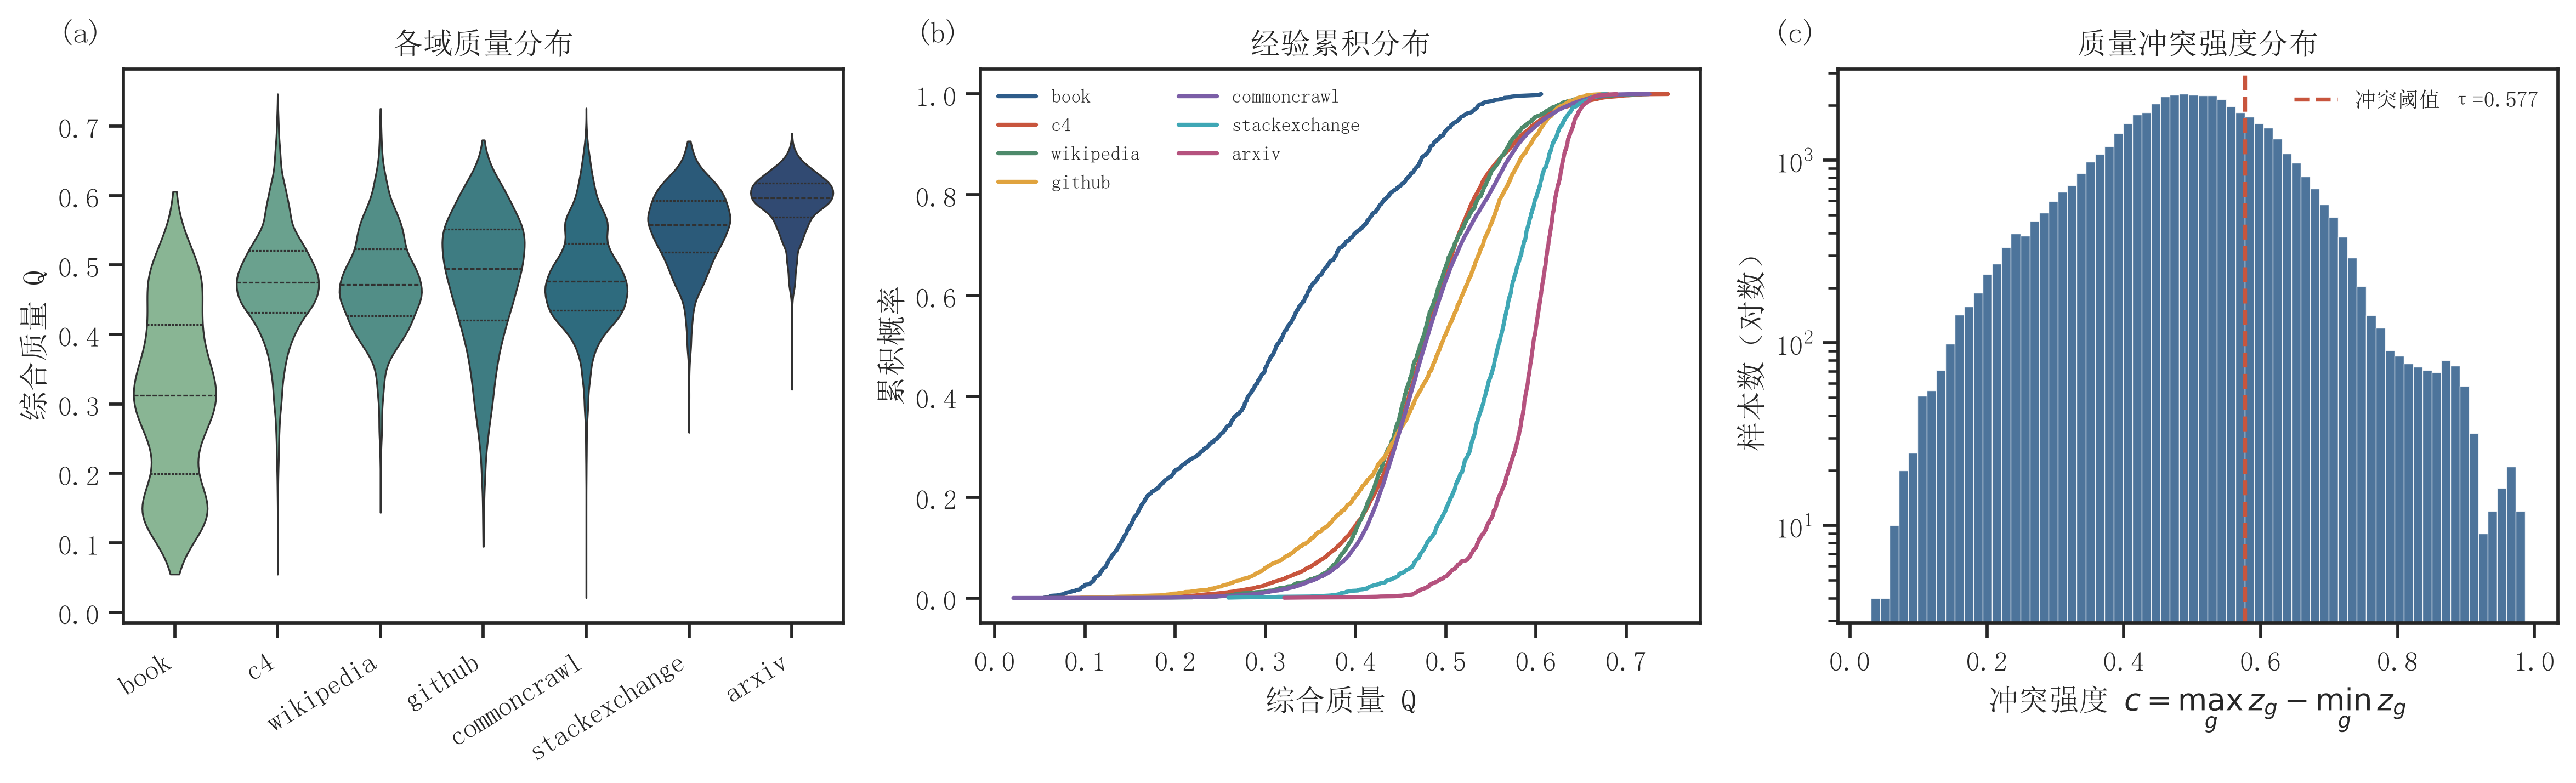
\includegraphics[width=0.95\textwidth]{figures/fig_q1_quality_dist.png}
\caption{各域质量分布、累积分布与冲突强度}
\label{fig:q1_dist}
\end{figure}

\begin{figure}[htbp]
\centering
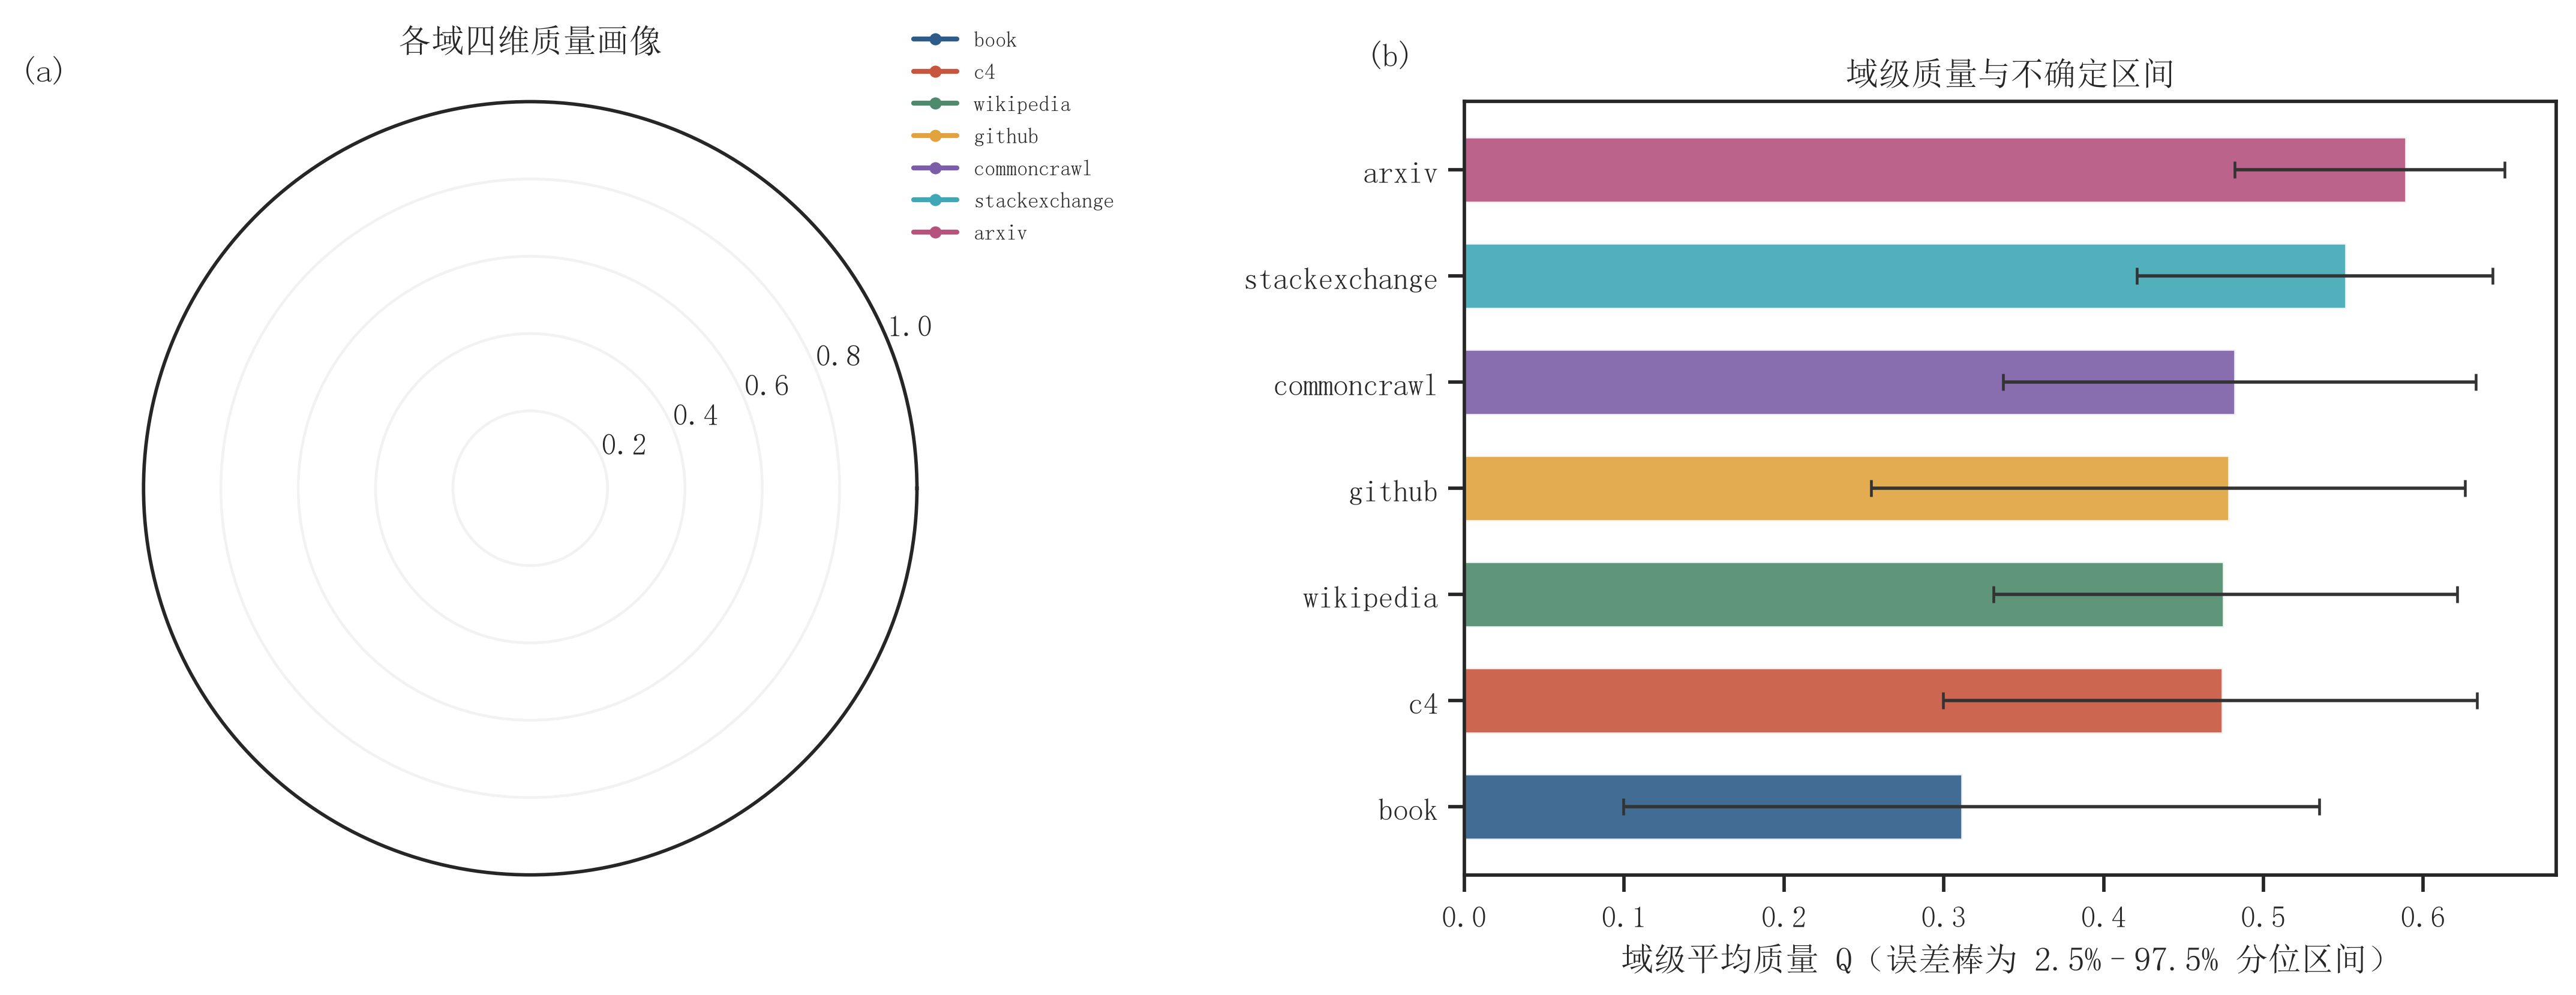
\includegraphics[width=0.92\textwidth]{figures/fig_q1_domain_quality.png}
\caption{域级质量画像与不确定区间}
\label{fig:q1_dom}
\end{figure}

结果呈现清晰的层次：学术类文本（arxiv、stackexchange）质量最高且一致性最好，网页抓取类（commoncrawl、c4）居中且内部离散度大，book 域质量最低但方差最大。图~\ref{fig:q1_dom}(a) 的雷达图进一步显示，book 在``低噪声''与``专业性''两维上明显塌陷，而其``教育价值''并不差——这正是它冲突率高达 83.3\% 的原因。

\subsubsection{聚合方式与敏感性}
\label{sec:q1_sens}

题面要求说明由样本向语料或领域的聚合方式。本文以\textbf{文档等权}为主口径，另报告按词数加权的对照。二者的差异很小（如 commoncrawl 为 0.482 对 0.477），说明域级结论不依赖于聚合权重。需说明的是，词数是按空格切分的粗略计数，\textbf{不能等同于 tokenizer 的 Token 数}，故仅作对照。

表~\ref{tab:q1_sens} 汇总了敏感性检验。ε 截断在三个量级上给出几乎相同的排序（秩相关 $\ge0.99999$）；标量化方式改用 softmax 期望后秩相关为 0.977，结论稳健。但\textbf{合成方式的影响很大}：改用等权算术平均后秩相关降至 0.665，用全指标几何平均降至 0.668。这说明``分组 + 组间几何平均''这一结构本身携带了信息，不是任意组合都能替代。

\begin{table}[htbp]
\centering
\caption{质量评分敏感性检验}
\label{tab:q1_sens}
\small
\begin{tabular}{l|l|r|r}
\toprule
\textbf{检验项} & \textbf{取值} & \textbf{与主结果秩相关} & \textbf{$Q$ 均值} \\
\midrule
\multirow{3}{*}{ε 截断} & $10^{-4}$ & 1.0000 & 0.482 \\
                        & $10^{-3}$（主） & 1.0000 & 0.482 \\
                        & $10^{-2}$ & 0.99999 & 0.483 \\
标量化方式 & softmax 期望 & 0.977 & 0.485 \\
\multirow{2}{*}{合成方式} & 等权算术平均 & 0.665 & 0.631 \\
                          & 全指标几何平均 & 0.668 & 0.427 \\
\bottomrule
\end{tabular}
\end{table}

\subsubsection{扩展集迁移检验}
\label{sec:q1_ext}

题面要求在扩展集上检验主要结论。本文将 A1 上\textbf{冻结}的归一化参数直接应用于两个扩展集，结果见表~\ref{tab:q1_ext}。

\begin{table}[htbp]
\centering
\caption{扩展集迁移检验（归一化参数在 A1 上冻结，不做任何重标定）}
\label{tab:q1_ext}
\small
\begin{tabular}{l|r|r|r|r|r}
\toprule
\textbf{扩展集} & \textbf{条数} & \textbf{域} & \textbf{扩展集平均 $Q$} & \textbf{A1 同域平均 $Q$} & \textbf{差异} \\
\midrule
A2 & 17\,438 & arxiv & 0.5874 & 0.5894 & $-0.0020$ \\
A3 & 187\,572 & github & 0.4803 & 0.4788 & $+0.0015$ \\
\bottomrule
\end{tabular}
\end{table}

两个扩展集的域级质量与 A1 同域的差异分别为 $-0.0020$ 与 $+0.0015$，冲突率的差异同样很小（arxiv 5.03\% 对 4.19\%，github 14.16\% 对 13.16\%）。A3 的样本量是 A1 中 github 域的 71 倍，仍给出几乎相同的域级质量，这一结果有力支持假设 2——\textbf{评分规则与归一化参数可以跨集迁移，域级质量是语料的稳定属性而非抽样偶然}。

\subsection{领域配比建模}

\subsubsection{模型形式}

配比 $p$ 位于单纯形上。由于 $\sum_i p_i=1$，完整二次多项式中的常数项与平方项与一次项不独立，会产生冗余。本文采用 Scheffé 规范形：

\begin{equation}
\widehat{L}_k(p)=\sum_{i=1}^{17}a_{ki}p_i+\sum_{i<j}b_{kij}\,p_ip_j,
\qquad k=1,\dots,13 .
\label{eq:mixture}
\end{equation}

共 17 个一次项与 $\binom{17}{2}=136$ 个交互项，每个目标域 153 个参数。训练样本仅 512 组，故引入岭惩罚：

\begin{equation}
\min_{a,b}\ \sum_{n}\left(L_{k}^{(n)}-\widehat{L}_k(p^{(n)})\right)^2
+\alpha\Big(\sum_i a_{ki}^2+\sum_{i<j}b_{kij}^2\Big),
\end{equation}

惩罚强度 $\alpha$ 由 A4/A5 上的 5 折交叉验证在 22 个对数网格点上选取。交互列乘以 17 以对齐量级，使惩罚对各列公平。评价目标为 13 个验证域的等权平均

\begin{equation}
L_{\mathrm{eval}}(p)=\sum_{k=1}^{13}v_k\widehat{L}_k(p),\qquad v_k=\tfrac{1}{13},
\end{equation}

权重 $v$ 固定且不随 $p$ 改变。需说明的是，17 个训练域中有 4 个（\texttt{nih\_exporter}、\texttt{enron\_emails}、\texttt{europarl}、\texttt{philpapers}）没有对应的验证损失列，它们仍作为配比输入参与建模，但不虚构其验证损失。

\subsubsection{二次项的价值}

表~\ref{tab:q1_mix} 与图~\ref{fig:q1_perf} 给出线性模型与二次混料模型的对比。二次项的引入把交叉验证 RMSE 从 0.283 降到 0.257，$R^2$ 从 0.240 提高到 0.375，Spearman 排序相关从 0.497 提高到 0.649。在保留的 1M 检验集上，二次模型的优势同样明显（RMSE 0.199 对 0.228，Spearman 0.701 对 0.624）。这说明领域之间确实存在\textbf{非加性的搭配效应}，不是简单线性叠加。

\begin{table}[htbp]
\centering
\caption{配比模型的交叉验证与检验集表现}
\label{tab:q1_mix}
\small
\begin{tabular}{l|l|r|r|r|r}
\toprule
\textbf{数据集} & \textbf{模型} & \textbf{RMSE} & \textbf{MAE} & \textbf{$R^2$} & \textbf{Spearman} \\
\midrule
\multirow{2}{*}{训练集 5 折 CV} & 线性混料 & 0.283 & 0.225 & 0.240 & 0.497 \\
                                & 二次混料 & \textbf{0.257} & \textbf{0.199} & \textbf{0.375} & \textbf{0.649} \\
\midrule
\multirow{2}{*}{1M 检验集 A6/A7} & 线性混料 & 0.228 & 0.181 & 0.327 & 0.624 \\
                                 & 二次混料 & \textbf{0.199} & \textbf{0.158} & \textbf{0.485} & \textbf{0.701} \\
\midrule
\multirow{2}{*}{60M 检验集 A8/A9} & 线性混料 & 1.520 & 1.508 & $-47.3$ & 0.558 \\
                                  & 二次混料 & \textbf{1.467} & \textbf{1.456} & $-43.9$ & \textbf{0.706} \\
\midrule
\multirow{2}{*}{1B 检验集 A10/A11} & 线性混料 & 3.194 & 3.190 & $-3782$ & 0.367 \\
                                   & 二次混料 & \textbf{2.830} & \textbf{2.822} & $-2968$ & \textbf{0.478} \\
\bottomrule
\end{tabular}
\end{table}

\begin{figure}[htbp]
\centering
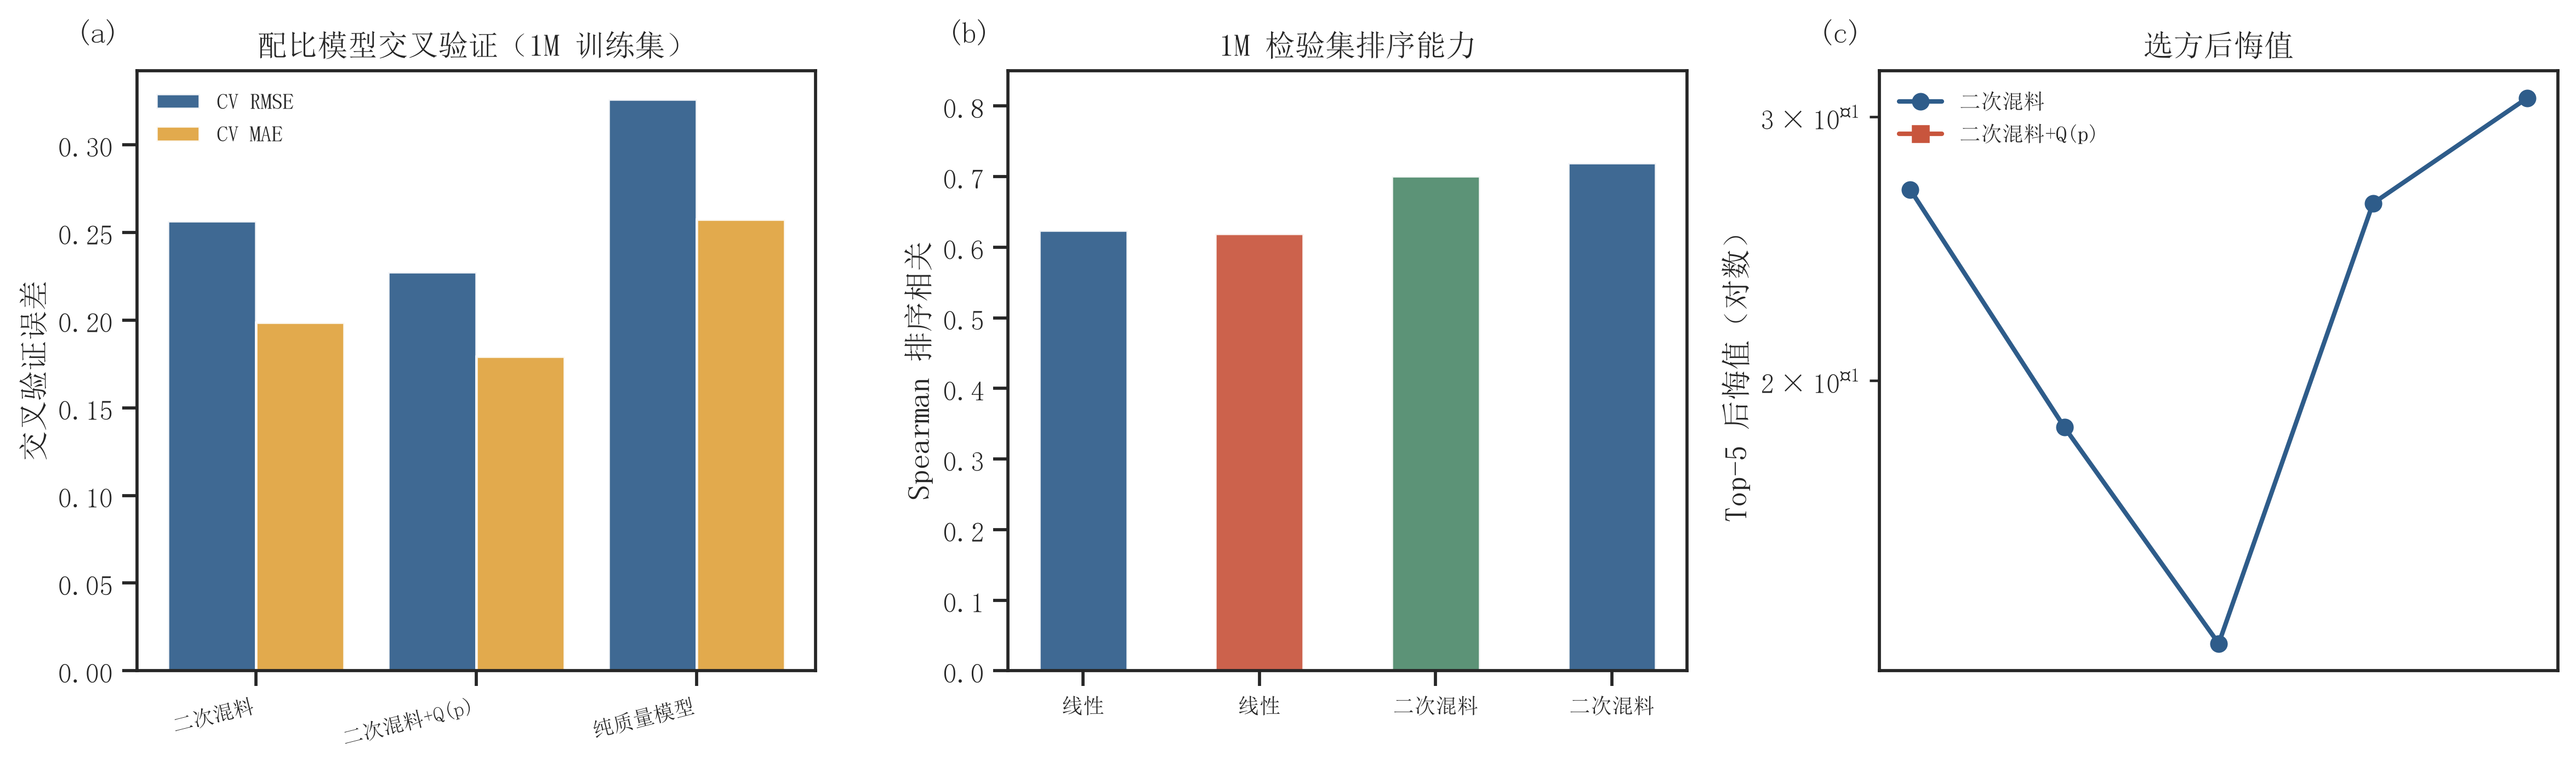
\includegraphics[width=0.95\textwidth]{figures/fig_q1_mixture_perf.png}
\caption{配比模型的交叉验证、排序能力与后悔值}
\label{fig:q1_perf}
\end{figure}

表~\ref{tab:q1_mix} 中 60M 与 1B 检验集的 $R^2$ 为大幅负值，这\textbf{不是模型失败，而是尺度不可比}：模型在 1M 规模的损失上训练，而 60M/1B 的损失绝对水平显著更低，直接套用会产生系统性偏差。因此对这两个检验集应当只看\textbf{排序指标}。二次模型在 60M 上的 Spearman 达 0.706，说明配比优劣的排序确实可以跨参数规模迁移。若在检验集的一半上拟合仿射尺度校准、在另一半上评估，二次模型在 60M 上的 RMSE 由 1.466 降至 0.161，进一步印证了偏差主要来自尺度而非排序。

\subsubsection{选方后悔值}

题面要求给出``预测最优配方的真实损失减去候选集真实最小损失''的后悔值。表~\ref{tab:q1_regret} 给出结果：在 1M 检验集上，二次模型的 Top-1 后悔值为 0.414，优于线性模型的 0.709；Top-5 后悔值 0.268 对 0.333。作为参照，随机选方的平均后悔值为 0.534。

\begin{table}[htbp]
\centering
\caption{选方后悔值（越低越好）}
\label{tab:q1_regret}
\small
\begin{tabular}{l|l|r|r|r|r}
\toprule
\textbf{检验集} & \textbf{模型} & \textbf{Top-1} & \textbf{Top-5} & \textbf{Top-10} & \textbf{随机选方} \\
\midrule
\multirow{2}{*}{1M} & 线性混料 & 0.709 & 0.333 & 0.262 & \multirow{2}{*}{0.534} \\
                    & 二次混料 & \textbf{0.414} & \textbf{0.268} & 0.268 & \\
\midrule
\multirow{2}{*}{60M} & 线性混料 & 0.618 & 0.299 & 0.217 & \multirow{2}{*}{0.380} \\
                     & 二次混料 & \textbf{0.288} & \textbf{0.186} & \textbf{0.175} & \\
\midrule
\multirow{2}{*}{1B} & 线性混料 & 0.116 & 0.120 & 0.103 & \multirow{2}{*}{0.114} \\
                    & 二次混料 & 0.333 & 0.134 & 0.102 & \\
\bottomrule
\end{tabular}
\end{table}

需要如实报告一个\textbf{负面结果}：在 1B 检验集上，二次模型的 Top-1 后悔值（0.333）反而高于线性模型（0.116），也高于随机选方。1B 检验集只有 64 个候选配方，Top-1 统计量本身波动很大，不宜据此下强结论；但这一现象提示二次模型在样本量小的场景下可能过拟合。在 10B/70B 外推表上，两个模型的 Spearman 秩相关均为负（$-0.45\sim-0.71$），说明\textbf{配比优劣的排序无法外推到数十亿参数以上}——这是外推表的固有局限（A12--A15 是由 1M/60M/1B 幂律外推生成的估算值，不是独立实验），本文不把它当作真实泛化证据。

\subsubsection{交互项的稳定性}

图~\ref{fig:q1_inter}(a) 给出交互项系数。用 bootstrap（200 次重采样）估计系数标准差后，1768 个交互系数中有 482 个（27.3\%）满足 $|b|/\mathrm{sd}>2$。这说明大约四分之一的搭配效应在不同重采样下稳定存在。但必须强调：\textbf{单个交互系数只表示相对该模型线性混合预测的偏离，不能直接读作``某两个领域互补/互斥''的因果结论}——要得到替代或互补的判断，还需做单纯形上的可行方向扰动，这部分放在\ref{sec:q2_subst}节与问题二一并讨论。

\begin{figure}[htbp]
\centering
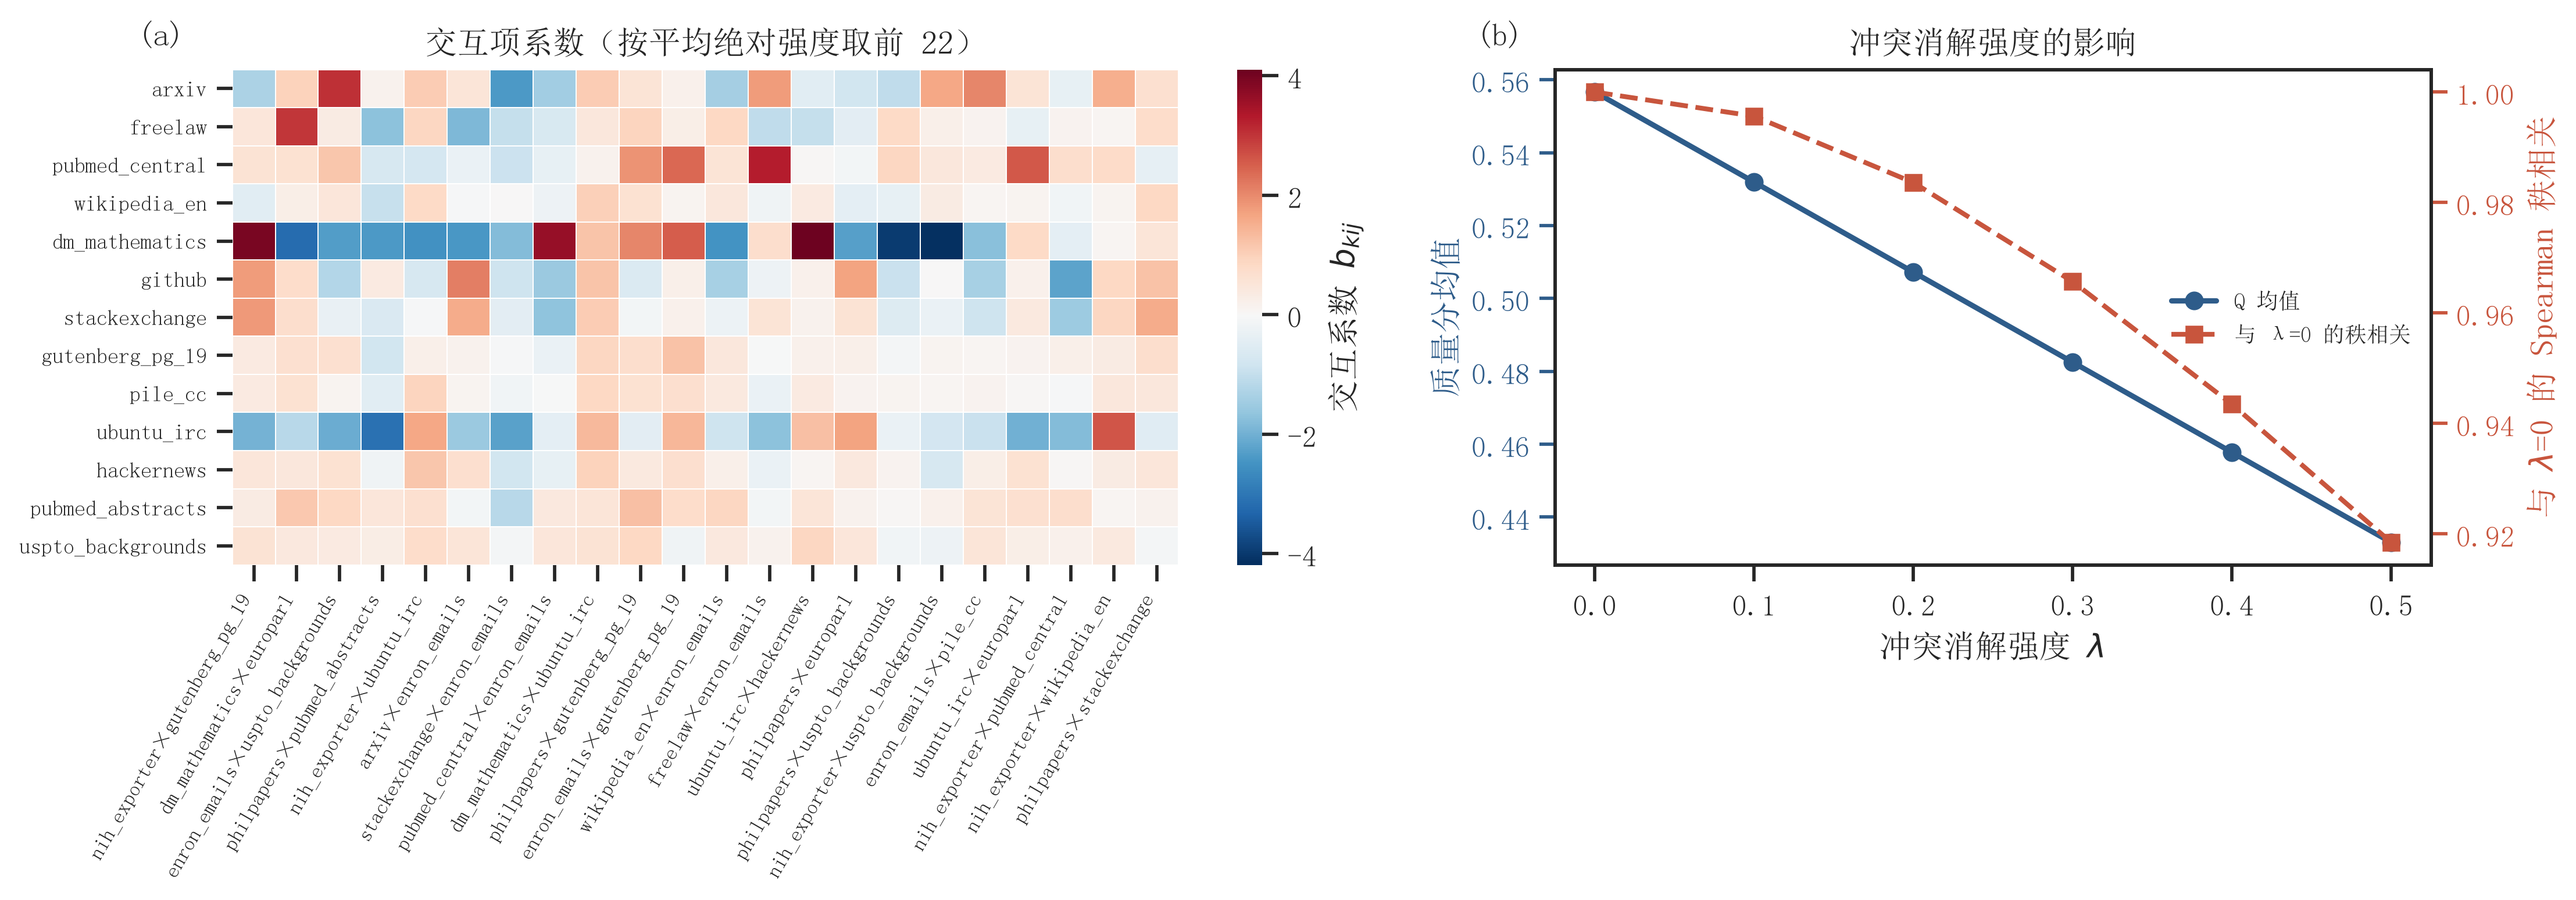
\includegraphics[width=0.95\textwidth]{figures/fig_q1_interaction.png}
\caption{交互项系数与冲突消解强度的敏感性}
\label{fig:q1_inter}
\end{figure}

\subsection{是否引入质量评分 $Q$：一个重要的识别问题}
\label{sec:q1_quality_in}

题面把``是否以及如何引入质量评分 $Q$''留给参赛队论证。本文对此做了专门检验，结论是\textbf{不应把 $Q$ 作为配比回归中的独立解释变量}，理由如下。

\subsubsection{完全共线}

若定义配比层面的综合质量

\begin{equation}
Q(p)=\sum_{i=1}^{17}p_iq_i,
\label{eq:Qp}
\end{equation}

其中 $q_i$ 为第 $i$ 个训练域的域级质量，则 $Q(p)$ 是 $p$ 的\textbf{线性函数}。用 17 个线性配比项回归 $Q(p)$，得 $R^2=1.0000000000$——完全共线。在无惩罚的最小二乘中，加入 $Q(p)$ 不提供任何新信息，其系数不可单独辨识。

\subsubsection{实证检验}

表~\ref{tab:q1_qaug} 给出三种模型在同一训练/检验切分下的表现：

\begin{table}[htbp]
\centering
\caption{引入 $Q(p)$ 的三种方式对比（5 折交叉验证）}
\label{tab:q1_qaug}
\small
\begin{tabular}{l|r|r|r|r|r}
\toprule
\textbf{模型} & \textbf{每域参数} & \textbf{CV RMSE} & \textbf{CV MAE} & \textbf{CV $R^2$} & \textbf{CV Spearman} \\
\midrule
二次混料（基准） & 153 & 0.257 & 0.199 & 0.375 & 0.649 \\
二次混料 $+\,Q(p)$ & 154 & \textbf{0.228} & \textbf{0.179} & \textbf{0.508} & \textbf{0.700} \\
纯质量模型 $a_k+c_kQ(p)$ & 2 & 0.326 & 0.258 & $-0.009$ & $-0.096$ \\
\bottomrule
\end{tabular}
\end{table}

\textbf{纯质量模型几乎完全没有预测能力}（$R^2=-0.009$，Spearman 为负），13 个目标域中只有 4 个的 $c_k$ 为负（即符合``质量越高损失越低''的预期）。这说明\textbf{单个质量标量无法承载配比与损失之间的关系}。

\textbf{加入 $Q(p)$ 确实改善了留出表现}（CV RMSE 0.257$\to$0.228，1M 检验 RMSE 0.199$\to$0.183），但由于存在完全共线，这一改善来自\textbf{岭惩罚结构的变化}而非新信息——$Q(p)$ 乘以 17 后作为一个特定线性组合被单独惩罚，等价于对原系数施加了一个有方向的收缩。因此\textbf{不能把 $c_k$ 解释为``质量的独立效应''}。

\subsubsection{结论}

质量信息应当通过问题二的有效数据量形式 $DQ^{\kappa}$ 进入模型，而不是作为配比回归的加性项。这既避免了共线性，又赋予质量与数据量可比量纲。本文后续采用这一路线。

\subsection{跨体系域映射}

两个域体系并不一一对应。A16 给出参考映射：arxiv、github、stackexchange 为 \texttt{direct}，wikipedia\_en$\to$wikipedia、gutenberg\_pg\_19$\to$book、pile\_cc$\to$commoncrawl 为 \texttt{near\_direct}，其余 11 个配方域没有同名质量域。本文按文本体裁为它们指定代理，映射规则与依据见表~\ref{tab:q1_map}。

\begin{table}[htbp]
\centering
\caption{配方域到质量域的映射与代理指派}
\label{tab:q1_map}
\small
\begin{tabular}{l|l|l|r}
\toprule
\textbf{配方域} & \textbf{质量域} & \textbf{映射类型} & \textbf{$q_i$} \\
\midrule
arxiv, github, stackexchange & 同名域 & direct & 0.589 / 0.479 / 0.552 \\
wikipedia\_en & wikipedia & near\_direct & 0.475 \\
gutenberg\_pg\_19 & book & near\_direct & 0.312 \\
pile\_cc & commoncrawl & near\_direct & 0.482 \\
dm\_mathematics, nih\_exporter, pubmed\_central, philpapers, pubmed\_abstracts, uspto\_backgrounds & arxiv & inferred\_proxy & 0.589 \\
ubuntu\_irc, hackernews & stackexchange & inferred\_proxy & 0.552 \\
freelaw, europarl & wikipedia & inferred\_proxy & 0.475 \\
enron\_emails & commoncrawl & inferred\_proxy & 0.482 \\
\bottomrule
\end{tabular}
\end{table}

代理指派的依据是文本体裁：学术论文全文与摘要归入 arxiv，技术问答与社区讨论归入 stackexchange，正式书面语归入 wikipedia，非正式日常文本归入 commoncrawl。得到 17 维质量向量 $q$，均值 0.527、范围 $[0.312,0.589]$。

\textbf{这一映射是建模假设而非已验证事实}：13 个域没有实测的质量信号，其 $q_i$ 值来自体裁代理。因此本文在后续只把 $q$ 用于构造 $Q(p)$ 这一\textbf{单调折算}，而不据此宣称任何域级的因果效应，并在敏感性分析中检验代理误差的影响。
